\doublespacing
\chap{Convolution Neural Network} 
\label{chap:CNN}
\section{Introduction}
Deep learning which is a branch of machine learning and artificial intelligence which is  inspired by the structure of the human brain. It  has made enormous strides in giving machines the ability to intuit the physical world. Convolutional Neural Networks are modeled around how living beings perceive world using their visual cortex. CNNs over the years have shown the ability to learn and extract complex features from images. In this work, we used this ability of convolutional neural network to generate features. In this chapter, we will look at basics of a neural network, starting with simple feed forward network and later delving into CNN.


\section{Neural Network}

The very basic definition of an artificial neural network is “a computer system modeled on the human brain and nervous system.”
\par
In very abstract terms, a neural network contains various neurons each having multiple inputs and importance of each input is given by its weight. A network of these neurons form neural network. We now look at the basic building blocks of a neural network.

\subsection{Neuron}
In nature a neuron consists of dendrites and  axons. The dendrites provide inputs to neuron from other neurons. After receiving the input, the neuron produces the output along the axons. The neuron sums up all the signals received from dendrites and activates based on some threshold value. 

\begin{figure}[H]
  \centering
    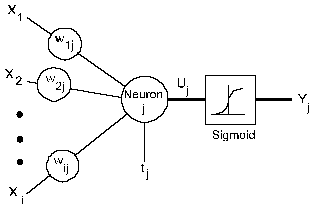
\includegraphics[scale=.3, angle=0]{Files/nn2.png}
    \caption[Single-layer Neural Networks (Perceptrons)]{Single-layer Neural Networks (Perceptrons)}
    \label{fig:NNNN}
\end{figure}


\par
Now that we are clear with the definition, we now explain fully feed forward neural network.
\section{Feed Forward Neural Network}
The feed forward neural network is an extension of the above concept. It consists of multiple layers, each layer has multiple neurons and information flows from input to the output. Important characteristics of a feed forward neural network is of not having any loop. Intuitively, feed forward neural network is a digraph containing neurons as nodes and weighted edges. To train a feed forward neural network the most popular technique is backpropagation.
\begin{figure}[H]
  \centering
    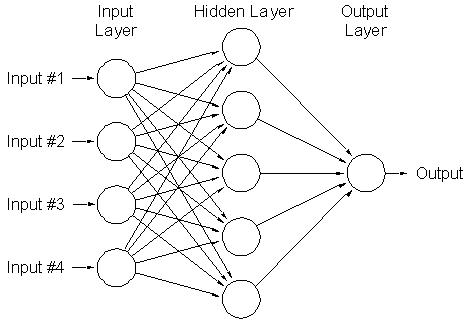
\includegraphics[scale=.6, angle=0]{Files/FFNN.png}
    \caption[Feed Forward Neural Network]{Feed Forward Neural Network}
    \label{fig:FFNN}
\end{figure}

\section{Backpropagation}
 Backprogation\cite{rumelhart1988learning} is an algorithm to find the local minima of an error function. In a feed forward neural network we have neurons and edges with weights which need to be fined tuned based on the output and error function.  The backpropagation algorithm computes the loss and uses  optimization algorithms such as gradient descent to propagate error in the backward direction recursively. This causes the change in weights of the edges which enables the whole network to adapt according to the data.  
\begin{figure}[H]
  \centering
    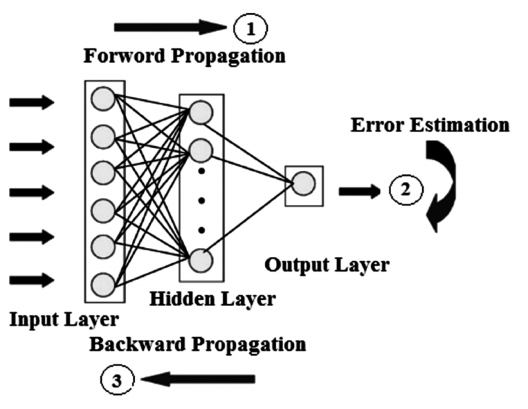
\includegraphics[scale=.4, angle=0]{Files/BackPropagation.png}
    \caption[Back Propagation Visualization]{Back Propagation Visualization}
    \label{fig:backpropogation}
\end{figure}

\section{Convolution Neural Network}

Convolution Neural Network are a variant of multi layer perceptron. inspired by the organization of the animal visual cortex. Convolution Neural Networks have repetitive blocks of neurons also known as features or kernels extending across the space. These repetitive blocks share weights during training. The CNN contains various types of layers, out of which the important layers are  as follows:

\subsection{Convolution}

Convolution is mathematical operation applied over two real valued arguments. Suppose we have two functions $f(x)$ and $h(x)$, then convolution operation over one dimension would be 

 \begin{equation}\label{eq:convolution-1d}
        \begin{aligned}
            g(x)=f(x) \ast h(x) = \int_{-\infty }^{\infty} f(s) \times h(x-s) ds
        \end{aligned}
\end{equation}

Here s is dummy integration variable. 
From the CNN and image perspective, our image becomes f(x) and kernel or feature map becomes h(x). The feature map is slided across the image and as it slides we apply the convolution operation over it to generate the output feature map. The values of these filters are fine tuned during training, but we have to decide the following key parameters commonly known as hyper-parameters before training.
\begin{itemize}
    \item  Depth corresponds to the number of filters or kernels mapped at any layer. In the \cref{fig:CNN} we can see that first layer we have 4 feature maps.
    \item Stride corresponds to the number of steps we take when we slide a feature map over the ouput from previous layer. For example, when we have set stride as 1 the, we slide filter on step and when we have set the stride as 3 the we slide the filter 3 steps each time.
\end{itemize}

\subsection{ Activation function}
Once convolution operation has been performed we apply a non linear activation function such as tanh, RELU, leakyRELU.

\subsection{Pooling}
Pooling is one the important building block of CNN. The main aim of the pooling operation is the reduction of feature maps by using some functions such taking maximum or minimum or average value of a subregions. Based on value of receptive field, the pooling operation is performed over the feature map obtained from the previous layer. For example, for a receptive field of value 3 and pooling function as average, we average a max value from every $3 \times 3$ area of feature map.

\begin{figure}[H]
  \centering
    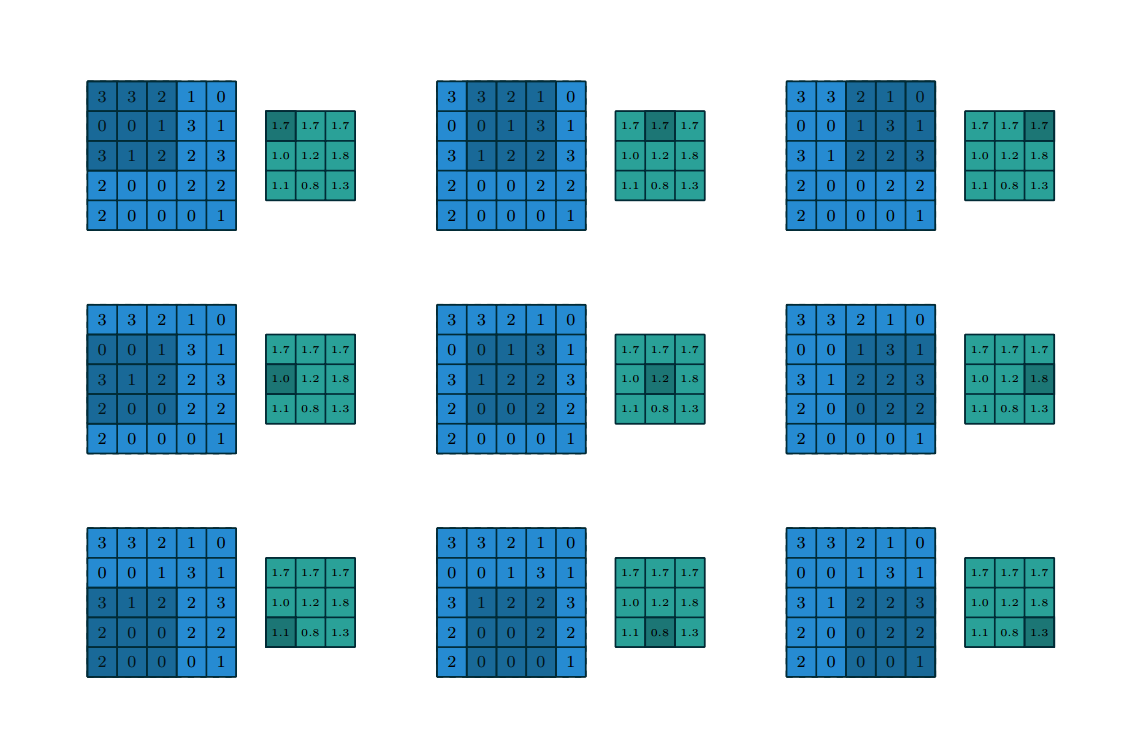
\includegraphics[scale=.3, angle=0]{Files/Pooling.png}
    \caption[Pooling Operation]{Computing output when $3 \times 3$ average pooling operation is performed \cite{1603.07285}}
    \label{fig:Pooling}
\end{figure}

\subsection{Fully Connected layer}
The last output layer is a fully connected layer over which various cost function such as sigmoid, soft-max are applied to generate the output.


\begin{figure}[H]
  \centering
    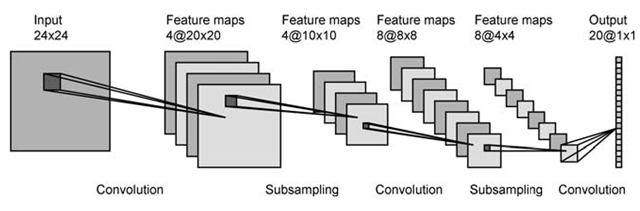
\includegraphics[scale=.6, angle=0]{Files/cnn-2.png}
    \caption[Convolutional Neural Network]{Convolutional Neural Network}
    \label{fig:CNN}
\end{figure}